\begin{figure*}[t]
  \begin{minipage}[t]{0.496\linewidth}
    \centering 
    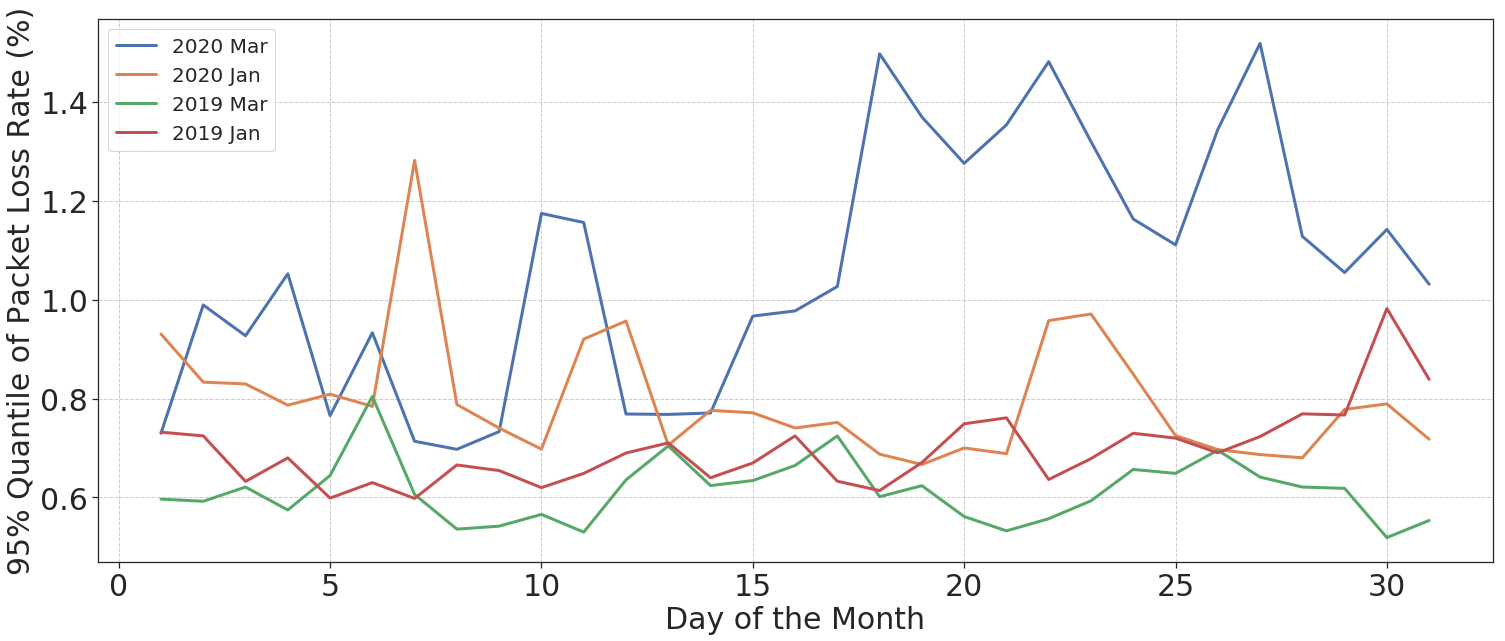
\includegraphics[width=0.98\linewidth]{figs/packet_loss_per_day.png} 
    \caption{Graph comparing the 95\% quantile packet loss per day for the month January, March 2019 and January, March 2020.} 
    \label{fig:packetlossperday} 
  \end{minipage}
  \begin{minipage}[t]{0.496\linewidth} 
    \centering 
    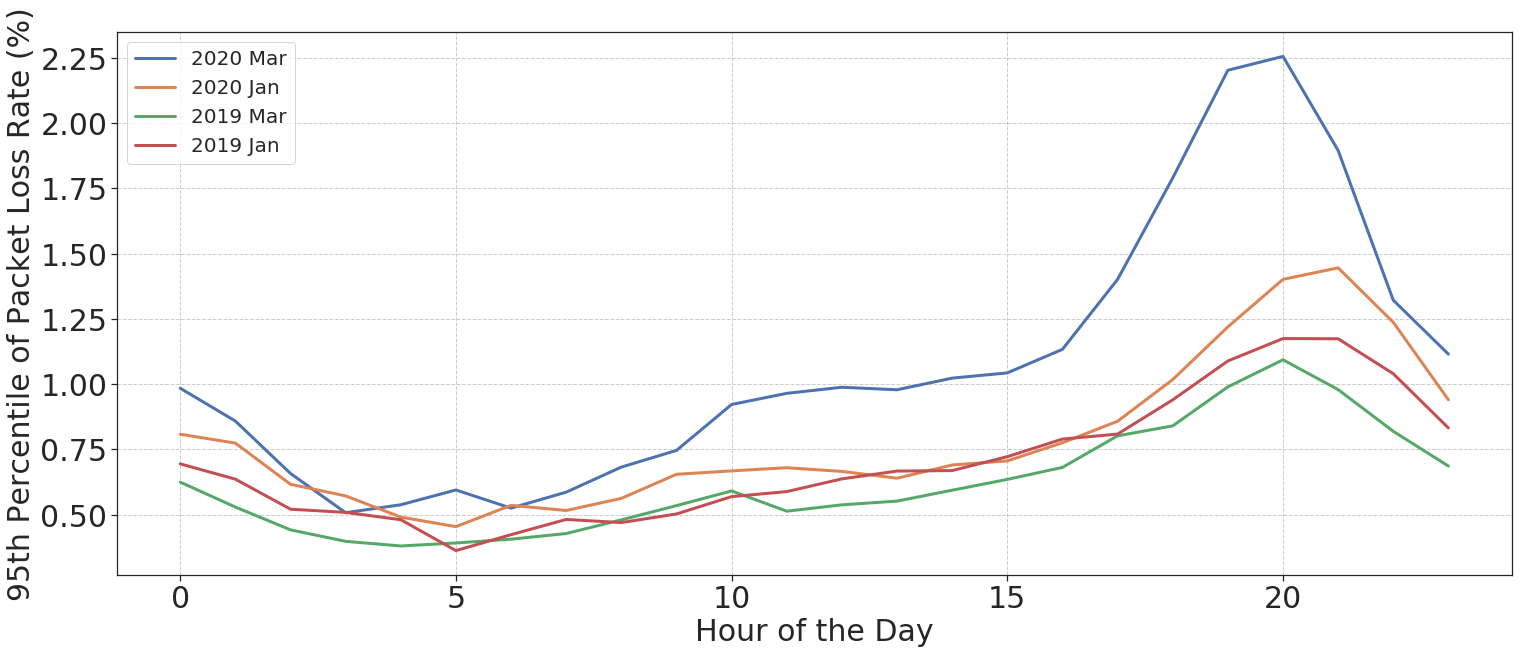
\includegraphics[width=0.98\linewidth]{figs/packet_loss_per_hour.png} 
    \caption{Graph comparing the 95\% quantile packet loss per hour for the month January, March 2019 and January, March 2020.} 
    \label{fig:packetlossperhour} 
  \end{minipage} 
\end{figure*}

\section{Packet Loss Analysis}
Apart from studying the data usage volume, we can also examine the effects of COVID-19 on  packet loss. As people were showing increased Internet usage during the lockdown period, potential network congestion might happen and can be reflected on the internet packet loss rate. To quantify the packet loss rate, we define the metric as:

\begin{equation}
    Packet \ Loss\, \% = \frac{\#Failure }{\#Failure + \#Success} \times 100
\end{equation}

We calculate the above for the $95\%$ quantile of all users as opposed to the average value, because we are more interested in studying the packet loss change from top users. We again shift the time to users' time zones locally.

\subsection{Daily Packet Loss}

% \begin{figure}[ht]
% \centering
% 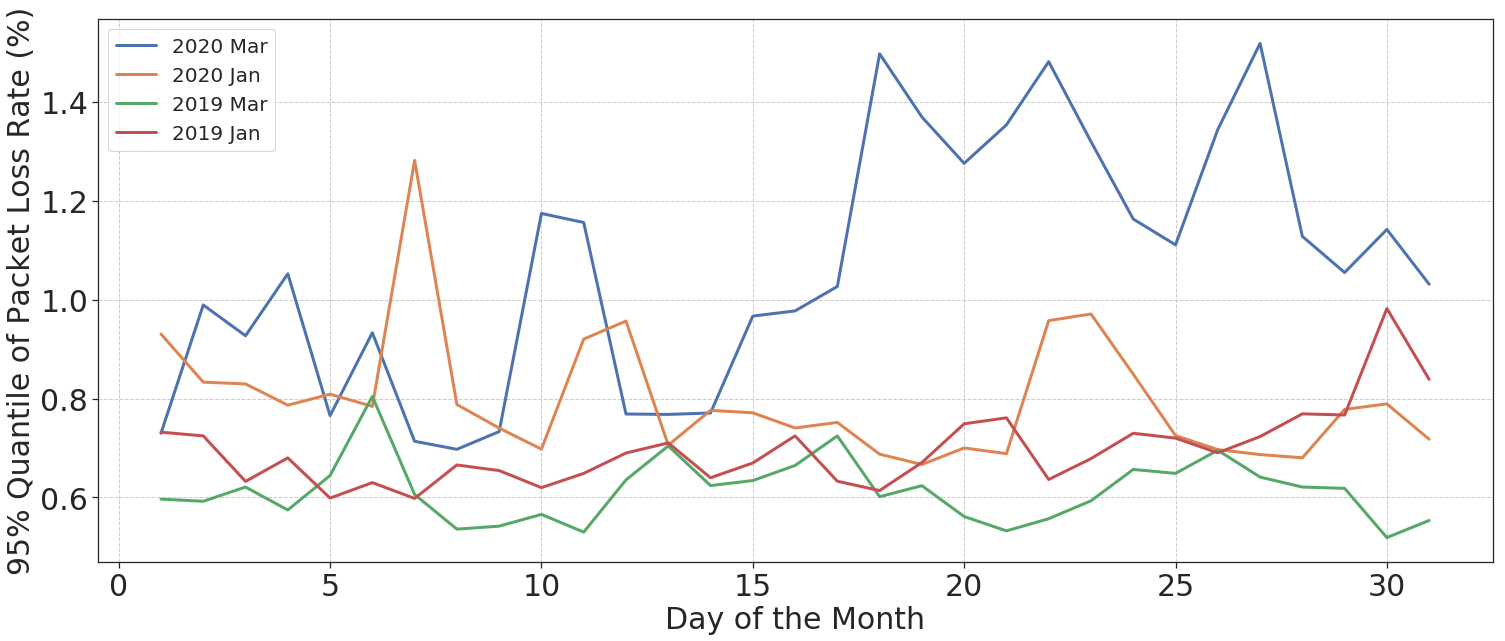
\includegraphics[width=1.0\linewidth]{figs/packet_loss_per_day.png}
% \caption{Graph comparing the 95\% quantile packet loss per day for the month January, March 2019 and January, March 2020.}
% \label{fig:packetlossperday}
% \end{figure}
  
We found a significant increase in packet loss starting from mid-March 2020 (Figure \ref{fig:packetlossperday}), the period when some states initiated lockdown policy. The growth of this packet loss rate showed more than 40--50\% compared to that of early March, which is before the pandemic. On late March 2020, packet loss percentage could be 80\% higher than that before the pandemic, implying that large traffic congestion might occur. Since we do not observe similar trend from the same month in 2019, this suggests that this increase is not due to noise and is instead due to activities such as tele-work. This increase also coincides with the increase in downloaded data we observed in metro areas in Figure \ref{fig:downloadmetro_rural}.

However, by the end of March, the loss rate again started to decrease compared to the highest level. We speculate that the rapid response of the network operations helped adjust the network capacity to the increasing need.

\subsection{Hourly Packet Loss}

% \begin{figure}[ht]
% \centering
% 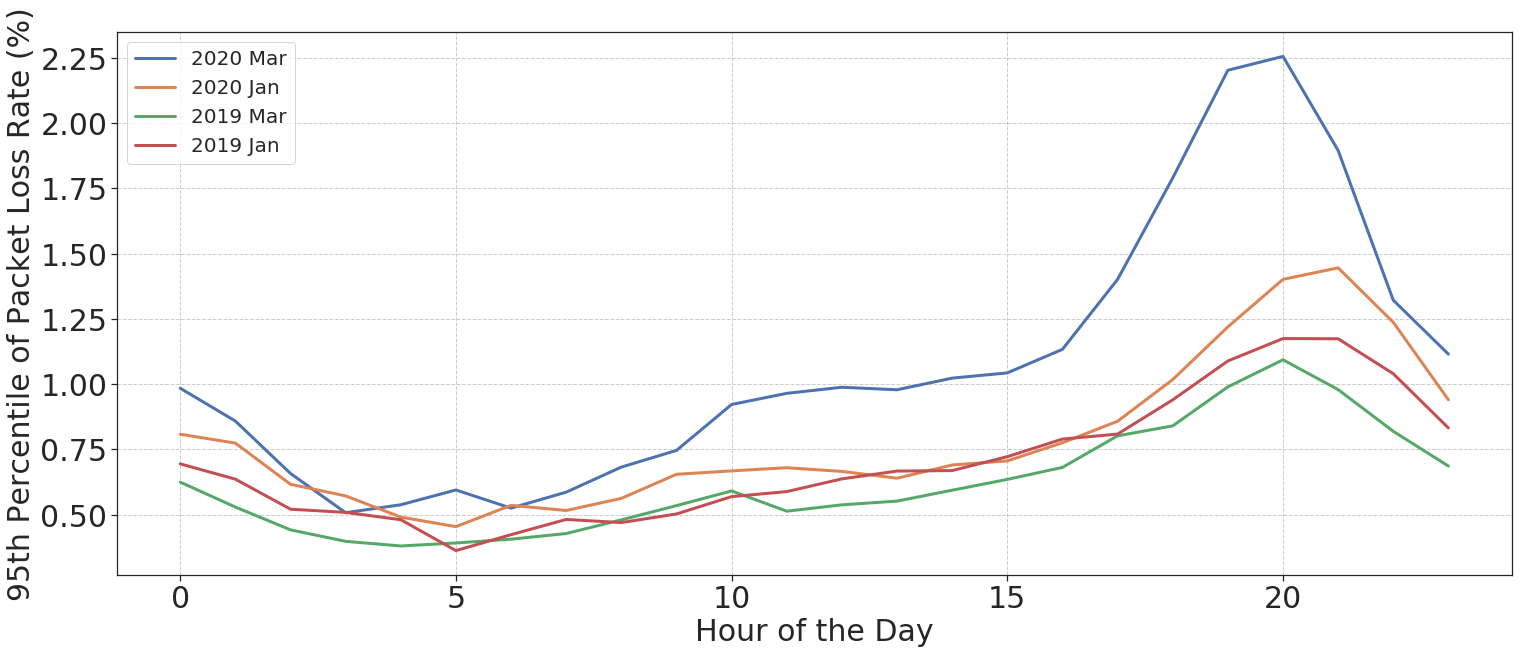
\includegraphics[width=1.0\linewidth]{figs/packet_loss_per_hour.png}
% \caption{Graph comparing the 95\% quantile packet loss per hour for the month January, March 2019 and January, March 2020.}
% \label{fig:packetlossperhour}
% \end{figure}

When considering the effect of the hour of the day, we found this packet loss change showed some shifts in hourly pattern as well, which again might be related to people's online activities.

As we discussed in the daily data section above, the hourly packet loss rate showed similar trend due to the daily patterns of users’ Internet behavior (Figure \ref{fig:packetlossperhour}). In March 2020, the packet loss rate increased steeply in the daytime from 7:00 to 22:00, potentially due to the users' growing online activities like remote learning, work from home, etc. However, this change was more evident during the evening. For example, we saw an around 59\% growth from 18:00 to 22:00 when comparing March to January 2020. This time period lies outside of traditional working hours - suggesting that packet loss is more positively related to the increased traffic due to recreational activities rather than remote working or distance learning. 

Our results are consistent with Candela et al. \cite{Candela2020latency}, as they found the increase of packet loss might be affected by factors like the type of target (whether belonging to a content delivery network or not), the version of the Internet Protocol, and the time of the day.


%\subsection{95\% Hourly Packet Loss}
%Besides, we notice the same slight increase of capacity loss through the hourly packet loss data.
